
\section{SNP calling}

%%%%%%%%%%%%%%%%%%%%%%%%%%%%%%%%%%%%%%%%%%%%%%%%%%%%%%%

\frame{
\frametitle{SNP calling procedures}

	\begin{figure}[!ht]
	\centering
	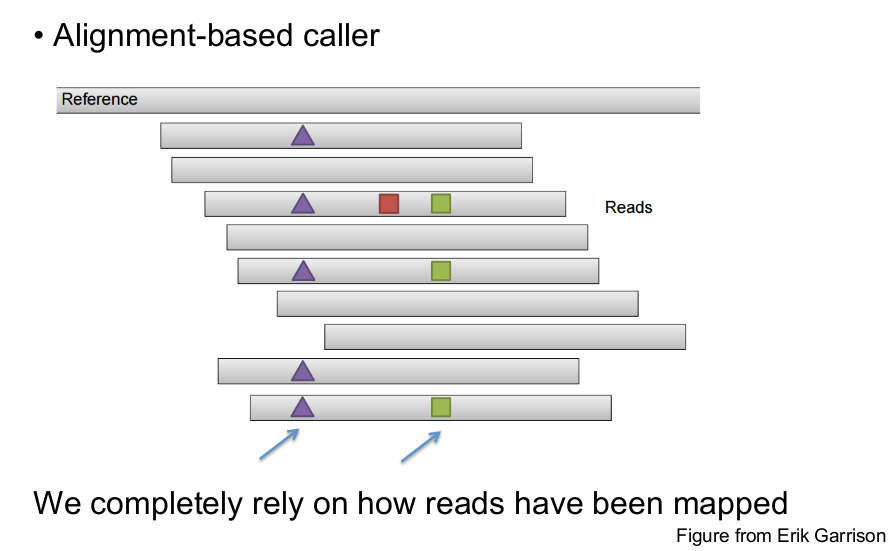
\includegraphics[width=9cm]{Pics/snp1.png}
	\end{figure}

}

%%%%%%%%%%%%%%%%%%%%%%%%%%%%%%%%%%%%%%%%%%%%%%%%%%%%%%%

\frame{
\frametitle{SNP calling procedures}

	\begin{figure}[!ht]
	\centering
	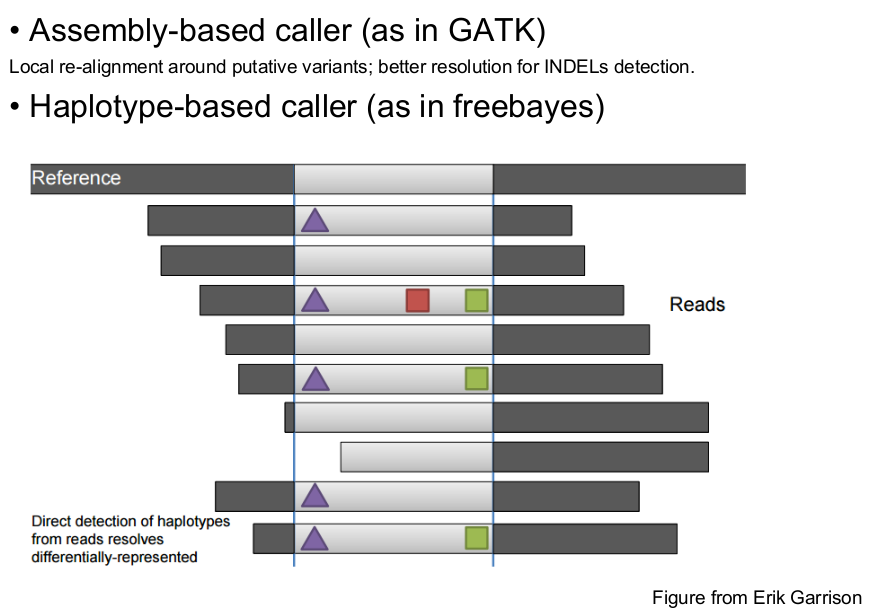
\includegraphics[width=9cm]{Pics/snp2.png}
	\end{figure}

}

%%%%%%%%%%%%%%%%%%%%%%%%%%%%%%%%%%%%%%%%%%%%%%%%%%%%%%%%%%

\frame{
\frametitle{Estimating allele frequencies}

	Assuming 2 alleles (A,G) with true allele frequency of 0.50

	\begin{center}
	\begin{tabular}{c|c|c|c}
	Sample & True genotype & Reads allele A & Read allele G\\
    \hline
    1 & AA & 7 & 0\\
    2 & AA & 25 & 1\\
    3 & AG & 5 & 3\\
    4 & AG & 4 & 4\\
    5 & GG & 0 & 2\\
    6 & GG & 0 & 4\\
    \hline
	\end{tabular}	
	\end{center}

	What is the simplest estimator of allele frequencies?

}


%%%%%%%%%%%%%%%%%%%%%%%%%%%%%%%%%%%%%%%%%%%%%%%%%%%%%%%%%%

\frame{
\frametitle{Estimating allele frequencies}

	Assuming 2 alleles (A,G) with true allele frequency of 0.50

	\begin{center}
	\begin{tabular}{c|c|c|c}
	Sample & True genotype & Reads allele A & Read allele G\\
    \hline
    1 & AA & 7 & 0\\
    2 & AA & 25 & 1\\
    3 & AG & 5 & 3\\
    4 & AG & 4 & 4\\
    5 & GG & 0 & 2\\
    6 & GG & 0 & 4\\
    \hline
    Total & & 41 & 14\\
    \hline
	\end{tabular}
	\end{center}

	\begin{equation*}
		\hat{f} = \frac{\sum_{i=1}^N n_{A,i}}{ \sum_{i=1}^N (n_{A,i}+n_{G,i}) }
	\end{equation*}

	$\hat{f}=0.75$

	What is wrong with this estimator?

}

%%%%%%%%%%%%%%%%%%%%%%%%%%%%%%%%%%%%%%%%%%%%%%%%%%%%%%%%%%

\frame{
\frametitle{Estimating allele frequencies}

	Assuming 2 alleles (A,G) with true allele frequency of 0.50

	\begin{center}
	\begin{tabular}{c|c|c|c}
	Sample & True genotype & Reads allele A & Read allele G\\
    \hline
    1 & AA & 7 & 0\\
    2 & AA & 25 & 1\\
    3 & AG & 5 & 3\\
    4 & AG & 4 & 4\\
    5 & GG & 0 & 2\\
    6 & GG & 0 & 4\\
    \hline
    Total & & 41 & 14\\
    \hline
	\end{tabular}
	\end{center}
    
    	\begin{equation*}
		\hat{n_A} = \sum_{i=1}^N (1-\epsilon)n_{A,i} + \epsilon n_{G,i} - \epsilon n_{A,i} - (1-\epsilon)n_{G,i}
	\end{equation*}
	
	%\begin{equation*}
	%	\hat{n_A}=\sum_{i=1}^N (1-\epsilon)(n_{A,i}-n_{G,i}) + \epsilon(n_{G,i}-n_{A,i})
	%\end{equation*}
    
    $\hat{f}=0.77$
}


%%%%%%%%%%%%%%%%%%%%%%%%%%%%%%%%%%%%%%%%%%%%%%%%%%%%%%%%%%

\frame{
\frametitle{Estimating allele frequencies}

	\begin{block}{Maximum Likelihood estimator}
		\begin{equation*}
			P(D|f) = \prod_{i=1}^N \sum_{g \in \{0,1,2\}} P(D|G=g) P(G=g|f)
		\end{equation*}
	\end{block}

}

%%%%%%%%%%%%%%%%%%%%%%%%%%%%%%%%%%%%%%%%%%%%%%%%%%%%%%%%%%

\frame{
\frametitle{Estimating allele frequencies}

        \begin{block}{Maximum Likelihood estimator}
                \begin{equation*}
                        P(D|f) = \prod_{i=1}^N \sum_{g \in \{0,1,2\}} P(D|G=g) P(G=g|f)
                \end{equation*}
        \end{block}

        $P(D|G=g)$ is the genotype likelihood and $P(G=g|f)$ is given by HWE (for instance).

	\begin{center}
        In our previous example, $\hat{f}=0.46$ which is much closer to the true value than previous estimators.
	\end{center}

}

%%%%%%%%%%%%%%%%%%%%%%%%%%%%%%%%%%%%%%%%%%%%%%%%%%%%%%%%%%%%%

\frame{
\frametitle{SNP calling}

	\begin{block}{Challenges}
	\begin{itemize}
	\item If high levels of missing data, then genotypes can be lost.
    \item Rare variants are hard to detect.
    \item Trade off between false positive and false negative rates.
	\end{itemize}
	\end{block}

	\begin{block}{How to call SNPs?}
	\begin{itemize}
	\item If at least one heterozygous genotype has been called.
    \item If the estimated allele frequency is above a certain threshold.
	\end{itemize}
	\end{block}


}


%%%%%%%%%%%%%%%%%%%%%%%%%%%%%%%%%%%%%%%%%%%%%%%%%%%%%%%%%%%%%

\frame{
\frametitle{SNP calling}

Call a SNP if
\begin{equation*}
	\hat{f} \geq t
\end{equation*}
where $t$ can be the minimum sample allele frequency detectable (e.g. $t=1/2N$ with $N$ diploids).

}


%%%%%%%%%%%%%%%%%%%%%%%%%%%%%%%%%%%%%%%%%%%%%%%%%%%%%%%%%%%%%

\frame{
\frametitle{Likelihood Ratio Test}

A Likelihood Ratio Test (LRT) compares the goodness	of fit between the null and the alternative model:
\begin{itemize}
\item Null model: $f=0$
\item Alternative model: $f \neq 0$
\end{itemize}

\begin{equation*}
T = -2 \log \frac{L(f=0)}{L(f=\hat{f}_{MLE})}
\end{equation*}

where $T$ is $\chi^2$ distributed with 1 degree of freedom.

}





